\documentclass[1p]{elsarticle_modified}
%\bibliographystyle{elsarticle-num}

%\usepackage[colorlinks]{hyperref}
%\usepackage{abbrmath_seonhwa} %\Abb, \Ascr, \Acal ,\Abf, \Afrak
\usepackage{amsfonts}
\usepackage{amssymb}
\usepackage{amsmath}
\usepackage{amsthm}
\usepackage{scalefnt}
\usepackage{amsbsy}
\usepackage{kotex}
\usepackage{caption}
\usepackage{subfig}
\usepackage{color}
\usepackage{graphicx}
\usepackage{xcolor} %% white, black, red, green, blue, cyan, magenta, yellow
\usepackage{float}
\usepackage{setspace}
\usepackage{hyperref}

\usepackage{tikz}
\usetikzlibrary{arrows}

\usepackage{multirow}
\usepackage{array} % fixed length table
\usepackage{hhline}

%%%%%%%%%%%%%%%%%%%%%
\makeatletter
\renewcommand*\env@matrix[1][\arraystretch]{%
	\edef\arraystretch{#1}%
	\hskip -\arraycolsep
	\let\@ifnextchar\new@ifnextchar
	\array{*\c@MaxMatrixCols c}}
\makeatother %https://tex.stackexchange.com/questions/14071/how-can-i-increase-the-line-spacing-in-a-matrix
%%%%%%%%%%%%%%%

\usepackage[normalem]{ulem}

\newcommand{\msout}[1]{\ifmmode\text{\sout{\ensuremath{#1}}}\else\sout{#1}\fi}
%SOURCE: \msout is \stkout macro in https://tex.stackexchange.com/questions/20609/strikeout-in-math-mode

\newcommand{\cancel}[1]{
	\ifmmode
	{\color{red}\msout{#1}}
	\else
	{\color{red}\sout{#1}}
	\fi
}

\newcommand{\add}[1]{
	{\color{blue}\uwave{#1}}
}

\newcommand{\replace}[2]{
	\ifmmode
	{\color{red}\msout{#1}}{\color{blue}\uwave{#2}}
	\else
	{\color{red}\sout{#1}}{\color{blue}\uwave{#2}}
	\fi
}

\newcommand{\Sol}{\mathcal{S}} %segment
\newcommand{\D}{D} %diagram
\newcommand{\A}{\mathcal{A}} %arc


%%%%%%%%%%%%%%%%%%%%%%%%%%%%%5 test

\def\sl{\operatorname{\textup{SL}}(2,\Cbb)}
\def\psl{\operatorname{\textup{PSL}}(2,\Cbb)}
\def\quan{\mkern 1mu \triangleright \mkern 1mu}

\theoremstyle{definition}
\newtheorem{thm}{Theorem}[section]
\newtheorem{prop}[thm]{Proposition}
\newtheorem{lem}[thm]{Lemma}
\newtheorem{ques}[thm]{Question}
\newtheorem{cor}[thm]{Corollary}
\newtheorem{defn}[thm]{Definition}
\newtheorem{exam}[thm]{Example}
\newtheorem{rmk}[thm]{Remark}
\newtheorem{alg}[thm]{Algorithm}

\newcommand{\I}{\sqrt{-1}}
\begin{document}

%\begin{frontmatter}
%
%\title{Boundary parabolic representations of knots up to 8 crossings}
%
%%% Group authors per affiliation:
%\author{Yunhi Cho} 
%\address{Department of Mathematics, University of Seoul, Seoul, Korea}
%\ead{yhcho@uos.ac.kr}
%
%
%\author{Seonhwa Kim} %\fnref{s_kim}}
%\address{Center for Geometry and Physics, Institute for Basic Science, Pohang, 37673, Korea}
%\ead{ryeona17@ibs.re.kr}
%
%\author{Hyuk Kim}
%\address{Department of Mathematical Sciences, Seoul National University, Seoul 08826, Korea}
%\ead{hyukkim@snu.ac.kr}
%
%\author{Seokbeom Yoon}
%\address{Department of Mathematical Sciences, Seoul National University, Seoul, 08826,  Korea}
%\ead{sbyoon15@snu.ac.kr}
%
%\begin{abstract}
%We find all boundary parabolic representation of knots up to 8 crossings.
%
%\end{abstract}
%\begin{keyword}
%    \MSC[2010] 57M25 
%\end{keyword}
%
%\end{frontmatter}

%\linenumbers
%\tableofcontents
%
\newcommand\colored[1]{\textcolor{white}{\rule[-0.35ex]{0.8em}{1.4ex}}\kern-0.8em\color{red} #1}%
%\newcommand\colored[1]{\textcolor{white}{ #1}\kern-2.17ex	\textcolor{white}{ #1}\kern-1.81ex	\textcolor{white}{ #1}\kern-2.15ex\color{red}#1	}

{\Large $\underline{12n_{0761}~(K12n_{0761})}$}

\setlength{\tabcolsep}{10pt}
\renewcommand{\arraystretch}{1.6}
\vspace{1cm}\begin{tabular}{m{100pt}>{\centering\arraybackslash}m{274pt}}
\multirow{5}{120pt}{
	\centering
	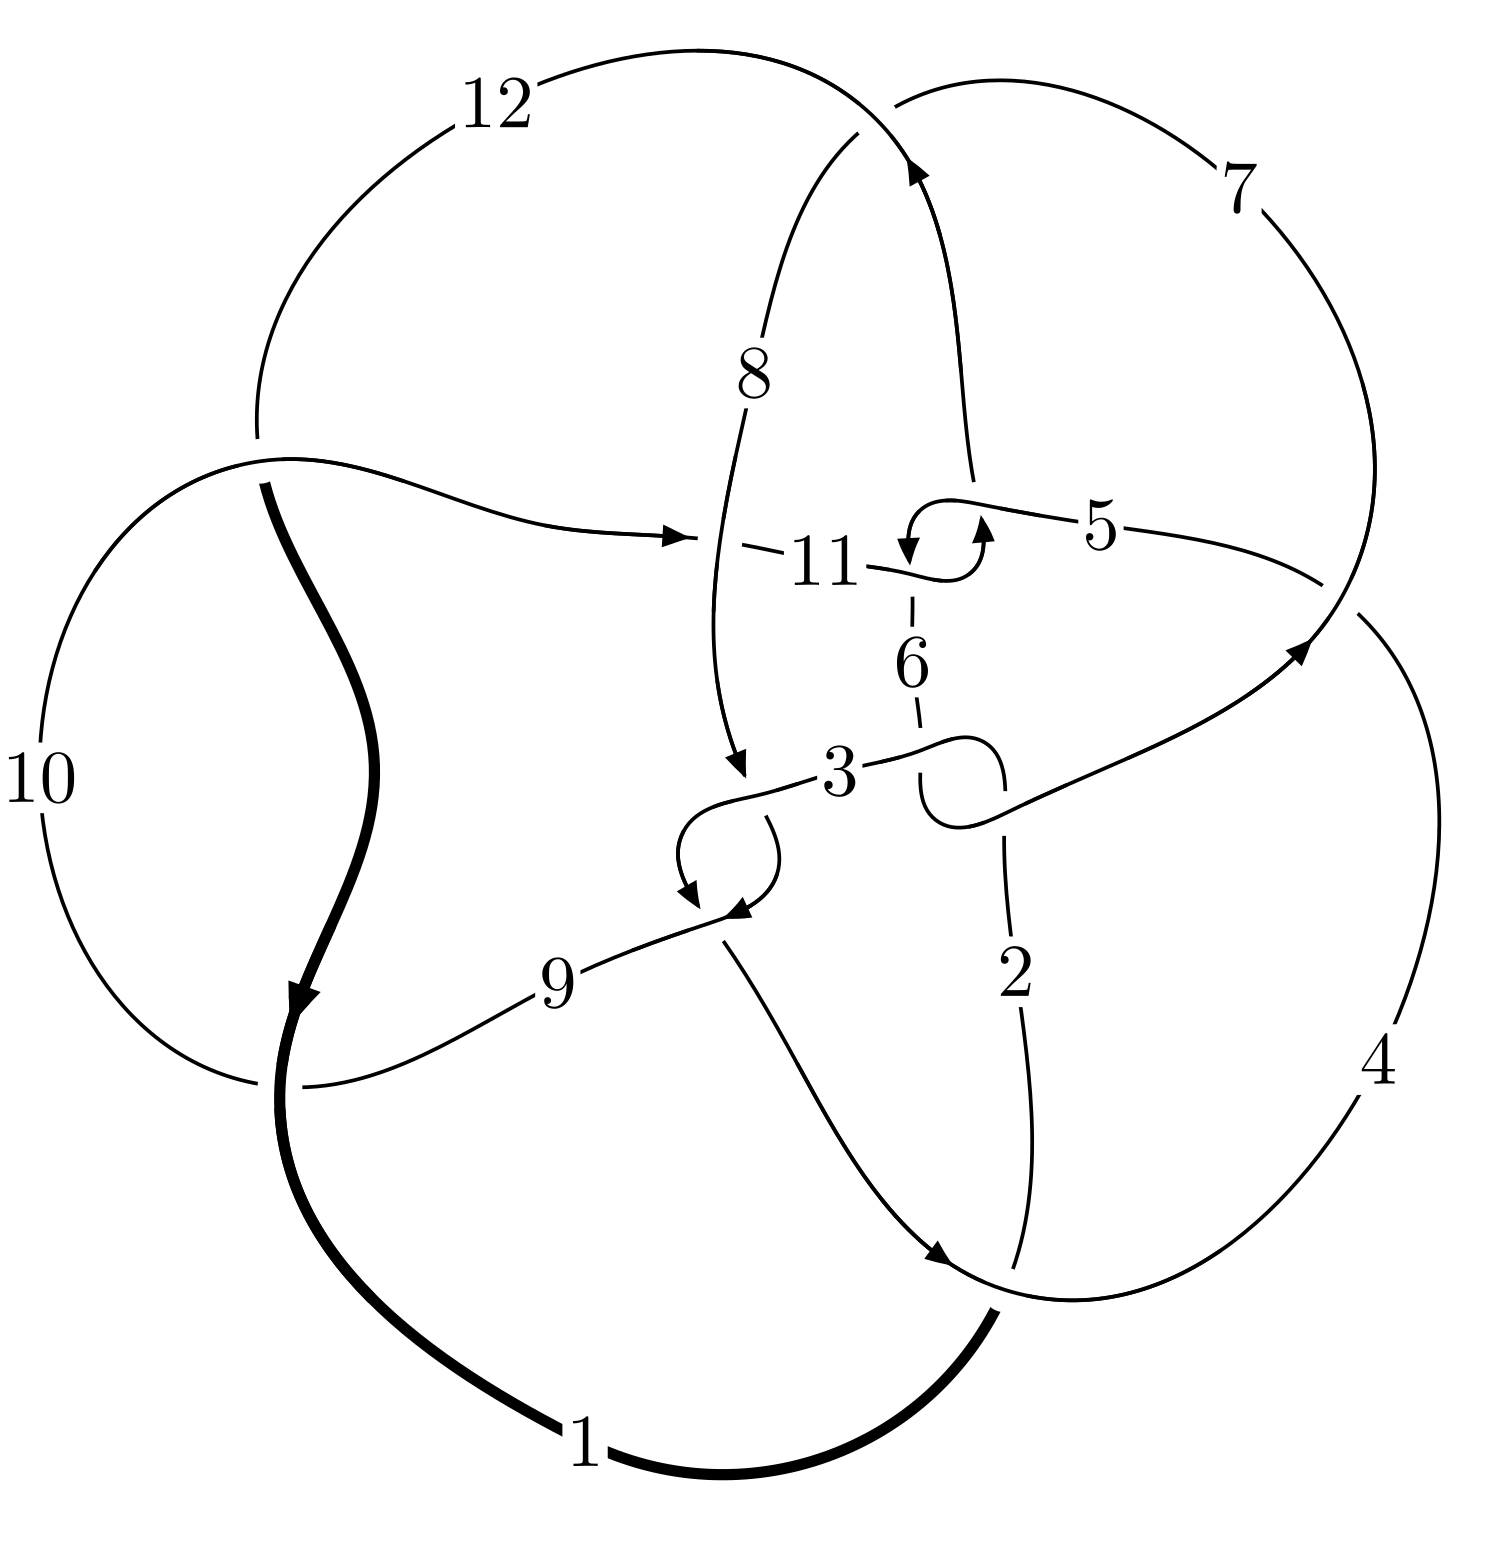
\includegraphics[width=112pt]{../../../GIT/diagram.site/Diagrams/png/2850_12n_0761.png}\\
\ \ \ A knot diagram\footnotemark}&
\allowdisplaybreaks
\textbf{Linearized knot diagam} \\
\cline{2-2}
 &
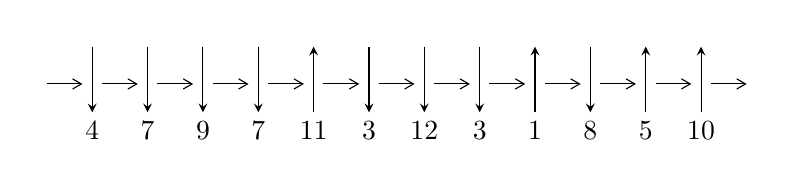
\begin{tikzpicture}[x=20pt, y=17pt]
	% nodes
	\node (C0) at (0, 0) {};
	\node (C1) at (1, 0) {};
	\node (C1U) at (1, +1) {};
	\node (C1D) at (1, -1) {4};

	\node (C2) at (2, 0) {};
	\node (C2U) at (2, +1) {};
	\node (C2D) at (2, -1) {7};

	\node (C3) at (3, 0) {};
	\node (C3U) at (3, +1) {};
	\node (C3D) at (3, -1) {9};

	\node (C4) at (4, 0) {};
	\node (C4U) at (4, +1) {};
	\node (C4D) at (4, -1) {7};

	\node (C5) at (5, 0) {};
	\node (C5U) at (5, +1) {};
	\node (C5D) at (5, -1) {11};

	\node (C6) at (6, 0) {};
	\node (C6U) at (6, +1) {};
	\node (C6D) at (6, -1) {3};

	\node (C7) at (7, 0) {};
	\node (C7U) at (7, +1) {};
	\node (C7D) at (7, -1) {12};

	\node (C8) at (8, 0) {};
	\node (C8U) at (8, +1) {};
	\node (C8D) at (8, -1) {3};

	\node (C9) at (9, 0) {};
	\node (C9U) at (9, +1) {};
	\node (C9D) at (9, -1) {1};

	\node (C10) at (10, 0) {};
	\node (C10U) at (10, +1) {};
	\node (C10D) at (10, -1) {8};

	\node (C11) at (11, 0) {};
	\node (C11U) at (11, +1) {};
	\node (C11D) at (11, -1) {5};

	\node (C12) at (12, 0) {};
	\node (C12U) at (12, +1) {};
	\node (C12D) at (12, -1) {10};
	\node (C13) at (13, 0) {};

	% arrows
	\draw[->,>={angle 60}]
	(C0) edge (C1) (C1) edge (C2) (C2) edge (C3) (C3) edge (C4) (C4) edge (C5) (C5) edge (C6) (C6) edge (C7) (C7) edge (C8) (C8) edge (C9) (C9) edge (C10) (C10) edge (C11) (C11) edge (C12) (C12) edge (C13) ;	\draw[->,>=stealth]
	(C1U) edge (C1D) (C2U) edge (C2D) (C3U) edge (C3D) (C4U) edge (C4D) (C5D) edge (C5U) (C6U) edge (C6D) (C7U) edge (C7D) (C8U) edge (C8D) (C9D) edge (C9U) (C10U) edge (C10D) (C11D) edge (C11U) (C12D) edge (C12U) ;
	\end{tikzpicture} \\
\hhline{~~} \\& 
\textbf{Solving Sequence} \\ \cline{2-2} 
 &
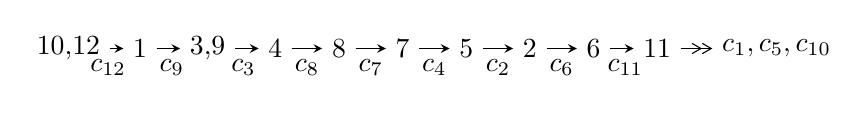
\begin{tikzpicture}[x=23pt, y=7pt]
	% node
	\node (A0) at (-1/8, 0) {10,12};
	\node (A1) at (1, 0) {1};
	\node (A2) at (33/16, 0) {3,9};
	\node (A3) at (25/8, 0) {4};
	\node (A4) at (33/8, 0) {8};
	\node (A5) at (41/8, 0) {7};
	\node (A6) at (49/8, 0) {5};
	\node (A7) at (57/8, 0) {2};
	\node (A8) at (65/8, 0) {6};
	\node (A9) at (73/8, 0) {11};
	\node (C1) at (1/2, -1) {$c_{12}$};
	\node (C2) at (3/2, -1) {$c_{9}$};
	\node (C3) at (21/8, -1) {$c_{3}$};
	\node (C4) at (29/8, -1) {$c_{8}$};
	\node (C5) at (37/8, -1) {$c_{7}$};
	\node (C6) at (45/8, -1) {$c_{4}$};
	\node (C7) at (53/8, -1) {$c_{2}$};
	\node (C8) at (61/8, -1) {$c_{6}$};
	\node (C9) at (69/8, -1) {$c_{11}$};
	\node (A10) at (11, 0) {$c_{1},c_{5},c_{10}$};

	% edge
	\draw[->,>=stealth]	
	(A0) edge (A1) (A1) edge (A2) (A2) edge (A3) (A3) edge (A4) (A4) edge (A5) (A5) edge (A6) (A6) edge (A7) (A7) edge (A8) (A8) edge (A9) ;
	\draw[->>,>={angle 60}]	
	(A9) edge (A10);
\end{tikzpicture} \\ 

\end{tabular} \\

\footnotetext{
The image of knot diagram is generated by the software ``\textbf{Draw programme}" developed by Andrew Bartholomew(\url{http://www.layer8.co.uk/maths/draw/index.htm\#Running-draw}), where we modified some parts for our purpose(\url{https://github.com/CATsTAILs/LinksPainter}).
}\phantom \\ \newline 
\centering \textbf{Ideals for irreducible components\footnotemark of $X_{\text{par}}$} 
 
\begin{align*}
I^u_{1}&=\langle 
3.97870\times10^{127} u^{63}+7.30559\times10^{127} u^{62}+\cdots+2.80101\times10^{129} b-2.17236\times10^{129},\\
\phantom{I^u_{1}}&\phantom{= \langle  }9.34021\times10^{128} u^{63}+2.00908\times10^{129} u^{62}+\cdots+2.80101\times10^{129} a+1.33402\times10^{131},\;u^{64}+2 u^{63}+\cdots+52 u-1\rangle \\
I^u_{2}&=\langle 
5.31075\times10^{16} u^{33}-2.70900\times10^{17} u^{32}+\cdots+1.01071\times10^{18} b+7.36359\times10^{17},\\
\phantom{I^u_{2}}&\phantom{= \langle  }-1.67036\times10^{19} u^{33}+2.51183\times10^{19} u^{32}+\cdots+5.55891\times10^{19} a+7.28093\times10^{19},\\
\phantom{I^u_{2}}&\phantom{= \langle  }u^{34}-3 u^{33}+\cdots-27 u+5\rangle \\
\\
\end{align*}
\raggedright * 2 irreducible components of $\dim_{\mathbb{C}}=0$, with total 98 representations.\\
\footnotetext{All coefficients of polynomials are rational numbers. But the coefficients are sometimes approximated in decimal forms when there is not enough margin.}
\newpage
\renewcommand{\arraystretch}{1}
\centering \section*{I. $I^u_{1}= \langle 3.98\times10^{127} u^{63}+7.31\times10^{127} u^{62}+\cdots+2.80\times10^{129} b-2.17\times10^{129},\;9.34\times10^{128} u^{63}+2.01\times10^{129} u^{62}+\cdots+2.80\times10^{129} a+1.33\times10^{131},\;u^{64}+2 u^{63}+\cdots+52 u-1 \rangle$}
\flushleft \textbf{(i) Arc colorings}\\
\begin{tabular}{m{7pt} m{180pt} m{7pt} m{180pt} }
\flushright $a_{10}=$&$\begin{pmatrix}0\\u\end{pmatrix}$ \\
\flushright $a_{12}=$&$\begin{pmatrix}1\\0\end{pmatrix}$ \\
\flushright $a_{1}=$&$\begin{pmatrix}1\\- u^2\end{pmatrix}$ \\
\flushright $a_{3}=$&$\begin{pmatrix}-0.333459 u^{63}-0.717269 u^{62}+\cdots-501.805 u-47.6263\\-0.0142045 u^{63}-0.0260820 u^{62}+\cdots-6.72756 u+0.775564\end{pmatrix}$ \\
\flushright $a_{9}=$&$\begin{pmatrix}- u\\u^3+u\end{pmatrix}$ \\
\flushright $a_{4}=$&$\begin{pmatrix}-0.345609 u^{63}-0.726001 u^{62}+\cdots-502.999 u-47.5965\\-0.0219766 u^{63}-0.0285431 u^{62}+\cdots-4.71159 u+0.730182\end{pmatrix}$ \\
\flushright $a_{8}=$&$\begin{pmatrix}1.02497 u^{63}+2.00739 u^{62}+\cdots+780.201 u+32.8037\\-0.0511564 u^{63}-0.107939 u^{62}+\cdots-26.5733 u-0.0850152\end{pmatrix}$ \\
\flushright $a_{7}=$&$\begin{pmatrix}0.973811 u^{63}+1.89945 u^{62}+\cdots+753.627 u+32.7187\\-0.0511564 u^{63}-0.107939 u^{62}+\cdots-26.5733 u-0.0850152\end{pmatrix}$ \\
\flushright $a_{5}=$&$\begin{pmatrix}-1.11384 u^{63}-2.14207 u^{62}+\cdots-740.710 u-40.0935\\0.0736073 u^{63}+0.141737 u^{62}+\cdots+25.8132 u+0.162424\end{pmatrix}$ \\
\flushright $a_{2}=$&$\begin{pmatrix}-0.163667 u^{63}-0.369101 u^{62}+\cdots-315.105 u-29.4435\\-0.0202597 u^{63}-0.0325595 u^{62}+\cdots-4.23987 u+0.489100\end{pmatrix}$ \\
\flushright $a_{6}=$&$\begin{pmatrix}1.29798 u^{63}+2.57666 u^{62}+\cdots+1114.78 u+53.0891\\-0.0501939 u^{63}-0.101574 u^{62}+\cdots-31.4978 u-0.323632\end{pmatrix}$ \\
\flushright $a_{11}=$&$\begin{pmatrix}-1.29596 u^{63}-2.48504 u^{62}+\cdots-761.398 u-18.2978\\0.0772814 u^{63}+0.139583 u^{62}+\cdots+40.7050 u-0.311959\end{pmatrix}$\\&\end{tabular}
\flushleft \textbf{(ii) Obstruction class $= -1$}\\~\\
\flushleft \textbf{(iii) Cusp Shapes $= -0.422995 u^{63}-0.770299 u^{62}+\cdots-106.004 u-6.77653$}\\~\\
\newpage\renewcommand{\arraystretch}{1}
\flushleft \textbf{(iv) u-Polynomials at the component}\newline \\
\begin{tabular}{m{50pt}|m{274pt}}
Crossings & \hspace{64pt}u-Polynomials at each crossing \\
\hline $$\begin{aligned}c_{1}\end{aligned}$$&$\begin{aligned}
&u^{64}-6 u^{63}+\cdots-11638 u+1297
\end{aligned}$\\
\hline $$\begin{aligned}c_{2},c_{6}\end{aligned}$$&$\begin{aligned}
&u^{64}+3 u^{63}+\cdots+274122 u+178861
\end{aligned}$\\
\hline $$\begin{aligned}c_{3},c_{8}\end{aligned}$$&$\begin{aligned}
&u^{64}- u^{63}+\cdots-514 u+43
\end{aligned}$\\
\hline $$\begin{aligned}c_{4}\end{aligned}$$&$\begin{aligned}
&u^{64}-7 u^{63}+\cdots+35883 u-2633
\end{aligned}$\\
\hline $$\begin{aligned}c_{5},c_{11}\end{aligned}$$&$\begin{aligned}
&u^{64}+u^{63}+\cdots-146 u-61
\end{aligned}$\\
\hline $$\begin{aligned}c_{7}\end{aligned}$$&$\begin{aligned}
&u^{64}+2 u^{63}+\cdots-1926 u-359
\end{aligned}$\\
\hline $$\begin{aligned}c_{9},c_{12}\end{aligned}$$&$\begin{aligned}
&u^{64}+2 u^{63}+\cdots+52 u-1
\end{aligned}$\\
\hline $$\begin{aligned}c_{10}\end{aligned}$$&$\begin{aligned}
&u^{64}-8 u^{63}+\cdots+360305 u-493889
\end{aligned}$\\
\hline
\end{tabular}\\~\\
\newpage\renewcommand{\arraystretch}{1}
\flushleft \textbf{(v) Riley Polynomials at the component}\newline \\
\begin{tabular}{m{50pt}|m{274pt}}
Crossings & \hspace{64pt}Riley Polynomials at each crossing \\
\hline $$\begin{aligned}c_{1}\end{aligned}$$&$\begin{aligned}
&y^{64}-102 y^{63}+\cdots-115080144 y+1682209
\end{aligned}$\\
\hline $$\begin{aligned}c_{2},c_{6}\end{aligned}$$&$\begin{aligned}
&y^{64}-97 y^{63}+\cdots-66879492684 y+31991257321
\end{aligned}$\\
\hline $$\begin{aligned}c_{3},c_{8}\end{aligned}$$&$\begin{aligned}
&y^{64}-65 y^{63}+\cdots-189118 y+1849
\end{aligned}$\\
\hline $$\begin{aligned}c_{4}\end{aligned}$$&$\begin{aligned}
&y^{64}-103 y^{63}+\cdots-1148483033 y+6932689
\end{aligned}$\\
\hline $$\begin{aligned}c_{5},c_{11}\end{aligned}$$&$\begin{aligned}
&y^{64}+61 y^{63}+\cdots-160274 y+3721
\end{aligned}$\\
\hline $$\begin{aligned}c_{7}\end{aligned}$$&$\begin{aligned}
&y^{64}-20 y^{63}+\cdots+12391674 y+128881
\end{aligned}$\\
\hline $$\begin{aligned}c_{9},c_{12}\end{aligned}$$&$\begin{aligned}
&y^{64}+56 y^{63}+\cdots-4566 y+1
\end{aligned}$\\
\hline $$\begin{aligned}c_{10}\end{aligned}$$&$\begin{aligned}
&y^{64}-36 y^{63}+\cdots-918166302603 y+243926344321
\end{aligned}$\\
\hline
\end{tabular}\\~\\
\newpage\flushleft \textbf{(vi) Complex Volumes and Cusp Shapes}
$$\begin{array}{c|c|c}  
\text{Solutions to }I^u_{1}& \I (\text{vol} + \sqrt{-1}CS) & \text{Cusp shape}\\
 \hline 
\begin{aligned}
u &= -1.007940 + 0.142695 I \\
a &= \phantom{-}1.72681 + 0.33227 I \\
b &= -2.14827 - 0.38605 I\end{aligned}
 & -5.44537 + 1.27224 I & \phantom{-0.000000 } 0 \\ \hline\begin{aligned}
u &= -1.007940 - 0.142695 I \\
a &= \phantom{-}1.72681 - 0.33227 I \\
b &= -2.14827 + 0.38605 I\end{aligned}
 & -5.44537 - 1.27224 I & \phantom{-0.000000 } 0 \\ \hline\begin{aligned}
u &= \phantom{-}0.249944 + 0.990791 I \\
a &= \phantom{-}0.640684 + 0.292773 I \\
b &= \phantom{-}1.131970 - 0.306003 I\end{aligned}
 & \phantom{-}0.77396 + 1.88121 I & \phantom{-0.000000 } 0 \\ \hline\begin{aligned}
u &= \phantom{-}0.249944 - 0.990791 I \\
a &= \phantom{-}0.640684 - 0.292773 I \\
b &= \phantom{-}1.131970 + 0.306003 I\end{aligned}
 & \phantom{-}0.77396 - 1.88121 I & \phantom{-0.000000 } 0 \\ \hline\begin{aligned}
u &= \phantom{-}0.550861 + 0.895713 I \\
a &= \phantom{-}0.776838 + 0.264285 I \\
b &= \phantom{-}0.537876 - 1.046190 I\end{aligned}
 & \phantom{-}0.74786 + 1.74560 I & \phantom{-0.000000 } 0 \\ \hline\begin{aligned}
u &= \phantom{-}0.550861 - 0.895713 I \\
a &= \phantom{-}0.776838 - 0.264285 I \\
b &= \phantom{-}0.537876 + 1.046190 I\end{aligned}
 & \phantom{-}0.74786 - 1.74560 I & \phantom{-0.000000 } 0 \\ \hline\begin{aligned}
u &= \phantom{-}0.249663 + 0.860286 I \\
a &= -0.007952 - 0.255517 I \\
b &= -1.346110 + 0.066798 I\end{aligned}
 & \phantom{-}1.46998 - 0.09365 I & -6.05569 - 0.75235 I \\ \hline\begin{aligned}
u &= \phantom{-}0.249663 - 0.860286 I \\
a &= -0.007952 + 0.255517 I \\
b &= -1.346110 - 0.066798 I\end{aligned}
 & \phantom{-}1.46998 + 0.09365 I & -6.05569 + 0.75235 I \\ \hline\begin{aligned}
u &= \phantom{-}0.816030 + 0.352936 I \\
a &= \phantom{-}1.065950 - 0.372916 I \\
b &= -1.21954 - 0.72193 I\end{aligned}
 & \phantom{-}1.34471 + 1.67458 I & \phantom{-}4.89337 - 2.28509 I \\ \hline\begin{aligned}
u &= \phantom{-}0.816030 - 0.352936 I \\
a &= \phantom{-}1.065950 + 0.372916 I \\
b &= -1.21954 + 0.72193 I\end{aligned}
 & \phantom{-}1.34471 - 1.67458 I & \phantom{-}4.89337 + 2.28509 I\\
 \hline 
 \end{array}$$\newpage$$\begin{array}{c|c|c}  
\text{Solutions to }I^u_{1}& \I (\text{vol} + \sqrt{-1}CS) & \text{Cusp shape}\\
 \hline 
\begin{aligned}
u &= \phantom{-}0.457483 + 1.043140 I \\
a &= \phantom{-}0.204342 + 0.373914 I \\
b &= \phantom{-}0.698972 - 0.215128 I\end{aligned}
 & -0.48463 + 2.79065 I & \phantom{-0.000000 } 0 \\ \hline\begin{aligned}
u &= \phantom{-}0.457483 - 1.043140 I \\
a &= \phantom{-}0.204342 - 0.373914 I \\
b &= \phantom{-}0.698972 + 0.215128 I\end{aligned}
 & -0.48463 - 2.79065 I & \phantom{-0.000000 } 0 \\ \hline\begin{aligned}
u &= -0.492479 + 1.105960 I \\
a &= \phantom{-}0.363473 - 0.562434 I \\
b &= \phantom{-}0.483288 + 0.305590 I\end{aligned}
 & -3.32128 - 6.55734 I & \phantom{-0.000000 } 0 \\ \hline\begin{aligned}
u &= -0.492479 - 1.105960 I \\
a &= \phantom{-}0.363473 + 0.562434 I \\
b &= \phantom{-}0.483288 - 0.305590 I\end{aligned}
 & -3.32128 + 6.55734 I & \phantom{-0.000000 } 0 \\ \hline\begin{aligned}
u &= \phantom{-}0.258616 + 1.235310 I \\
a &= \phantom{-}1.77466 - 1.22348 I \\
b &= -0.172078 - 0.546913 I\end{aligned}
 & -16.2576 + 2.1070 I & \phantom{-0.000000 } 0 \\ \hline\begin{aligned}
u &= \phantom{-}0.258616 - 1.235310 I \\
a &= \phantom{-}1.77466 + 1.22348 I \\
b &= -0.172078 + 0.546913 I\end{aligned}
 & -16.2576 - 2.1070 I & \phantom{-0.000000 } 0 \\ \hline\begin{aligned}
u &= \phantom{-}0.696765 + 0.232307 I \\
a &= -1.16792 + 1.33211 I \\
b &= \phantom{-}0.171332 - 0.345569 I\end{aligned}
 & -13.19110 + 1.27884 I & -7.41673 - 0.45833 I \\ \hline\begin{aligned}
u &= \phantom{-}0.696765 - 0.232307 I \\
a &= -1.16792 - 1.33211 I \\
b &= \phantom{-}0.171332 + 0.345569 I\end{aligned}
 & -13.19110 - 1.27884 I & -7.41673 + 0.45833 I \\ \hline\begin{aligned}
u &= -0.682790 + 0.263870 I \\
a &= \phantom{-}0.438693 - 0.369280 I \\
b &= -0.342223 + 0.086473 I\end{aligned}
 & -0.95985 + 2.04685 I & -1.75065 - 3.12369 I \\ \hline\begin{aligned}
u &= -0.682790 - 0.263870 I \\
a &= \phantom{-}0.438693 + 0.369280 I \\
b &= -0.342223 - 0.086473 I\end{aligned}
 & -0.95985 - 2.04685 I & -1.75065 + 3.12369 I\\
 \hline 
 \end{array}$$\newpage$$\begin{array}{c|c|c}  
\text{Solutions to }I^u_{1}& \I (\text{vol} + \sqrt{-1}CS) & \text{Cusp shape}\\
 \hline 
\begin{aligned}
u &= -0.174623 + 1.260770 I \\
a &= -2.35850 + 0.45076 I \\
b &= -1.53794 - 0.61406 I\end{aligned}
 & -11.49590 + 1.71321 I & \phantom{-0.000000 } 0 \\ \hline\begin{aligned}
u &= -0.174623 - 1.260770 I \\
a &= -2.35850 - 0.45076 I \\
b &= -1.53794 + 0.61406 I\end{aligned}
 & -11.49590 - 1.71321 I & \phantom{-0.000000 } 0 \\ \hline\begin{aligned}
u &= -0.306605 + 1.249510 I \\
a &= \phantom{-}0.200371 + 0.206893 I \\
b &= \phantom{-}0.627190 + 0.049373 I\end{aligned}
 & -5.37789 - 1.23730 I & \phantom{-0.000000 } 0 \\ \hline\begin{aligned}
u &= -0.306605 - 1.249510 I \\
a &= \phantom{-}0.200371 - 0.206893 I \\
b &= \phantom{-}0.627190 - 0.049373 I\end{aligned}
 & -5.37789 + 1.23730 I & \phantom{-0.000000 } 0 \\ \hline\begin{aligned}
u &= -1.285920 + 0.192101 I \\
a &= -1.42596 - 0.15956 I \\
b &= \phantom{-}2.57629 - 0.75755 I\end{aligned}
 & -15.2764 - 8.8264 I & \phantom{-0.000000 } 0 \\ \hline\begin{aligned}
u &= -1.285920 - 0.192101 I \\
a &= -1.42596 + 0.15956 I \\
b &= \phantom{-}2.57629 + 0.75755 I\end{aligned}
 & -15.2764 + 8.8264 I & \phantom{-0.000000 } 0 \\ \hline\begin{aligned}
u &= -0.656758\phantom{ +0.000000I} \\
a &= -1.69115\phantom{ +0.000000I} \\
b &= \phantom{-}0.229294\phantom{ +0.000000I}\end{aligned}
 & -7.54151\phantom{ +0.000000I} & -19.1290\phantom{ +0.000000I} \\ \hline\begin{aligned}
u &= \phantom{-}0.030952 + 1.346990 I \\
a &= -0.59570 - 1.40447 I \\
b &= -0.841490 - 0.064539 I\end{aligned}
 & -5.51440 + 0.30301 I & \phantom{-0.000000 } 0 \\ \hline\begin{aligned}
u &= \phantom{-}0.030952 - 1.346990 I \\
a &= -0.59570 + 1.40447 I \\
b &= -0.841490 + 0.064539 I\end{aligned}
 & -5.51440 - 0.30301 I & \phantom{-0.000000 } 0 \\ \hline\begin{aligned}
u &= \phantom{-}0.016235 + 1.351670 I \\
a &= -0.74947 + 1.55560 I \\
b &= -0.902586 + 0.406360 I\end{aligned}
 & -8.88905 + 3.84557 I & \phantom{-0.000000 } 0\\
 \hline 
 \end{array}$$\newpage$$\begin{array}{c|c|c}  
\text{Solutions to }I^u_{1}& \I (\text{vol} + \sqrt{-1}CS) & \text{Cusp shape}\\
 \hline 
\begin{aligned}
u &= \phantom{-}0.016235 - 1.351670 I \\
a &= -0.74947 - 1.55560 I \\
b &= -0.902586 - 0.406360 I\end{aligned}
 & -8.88905 - 3.84557 I & \phantom{-0.000000 } 0 \\ \hline\begin{aligned}
u &= \phantom{-}0.895451 + 1.019690 I \\
a &= \phantom{-}0.417165 + 0.878340 I \\
b &= \phantom{-}1.62581 - 2.01395 I\end{aligned}
 & \phantom{-}0.31944 + 4.24899 I & \phantom{-0.000000 } 0 \\ \hline\begin{aligned}
u &= \phantom{-}0.895451 - 1.019690 I \\
a &= \phantom{-}0.417165 - 0.878340 I \\
b &= \phantom{-}1.62581 + 2.01395 I\end{aligned}
 & \phantom{-}0.31944 - 4.24899 I & \phantom{-0.000000 } 0 \\ \hline\begin{aligned}
u &= -0.387601 + 1.301540 I \\
a &= -0.48828 - 2.11903 I \\
b &= \phantom{-}1.79526 - 0.66734 I\end{aligned}
 & -9.22324 - 6.23066 I & \phantom{-0.000000 } 0 \\ \hline\begin{aligned}
u &= -0.387601 - 1.301540 I \\
a &= -0.48828 + 2.11903 I \\
b &= \phantom{-}1.79526 + 0.66734 I\end{aligned}
 & -9.22324 + 6.23066 I & \phantom{-0.000000 } 0 \\ \hline\begin{aligned}
u &= -0.254005 + 1.347870 I \\
a &= \phantom{-}0.707175 + 1.216390 I \\
b &= -0.250688 + 0.217652 I\end{aligned}
 & -11.89940 - 3.29862 I & \phantom{-0.000000 } 0 \\ \hline\begin{aligned}
u &= -0.254005 - 1.347870 I \\
a &= \phantom{-}0.707175 - 1.216390 I \\
b &= -0.250688 - 0.217652 I\end{aligned}
 & -11.89940 + 3.29862 I & \phantom{-0.000000 } 0 \\ \hline\begin{aligned}
u &= -0.089807 + 1.382760 I \\
a &= -0.33602 + 1.52963 I \\
b &= -0.830903 + 0.034127 I\end{aligned}
 & -9.26019 - 5.11499 I & \phantom{-0.000000 } 0 \\ \hline\begin{aligned}
u &= -0.089807 - 1.382760 I \\
a &= -0.33602 - 1.52963 I \\
b &= -0.830903 - 0.034127 I\end{aligned}
 & -9.26019 + 5.11499 I & \phantom{-0.000000 } 0 \\ \hline\begin{aligned}
u &= \phantom{-}0.142080 + 1.389040 I \\
a &= -0.957401 + 0.071022 I \\
b &= -1.53212 + 0.09517 I\end{aligned}
 & -7.50523 + 2.04977 I & \phantom{-0.000000 } 0\\
 \hline 
 \end{array}$$\newpage$$\begin{array}{c|c|c}  
\text{Solutions to }I^u_{1}& \I (\text{vol} + \sqrt{-1}CS) & \text{Cusp shape}\\
 \hline 
\begin{aligned}
u &= \phantom{-}0.142080 - 1.389040 I \\
a &= -0.957401 - 0.071022 I \\
b &= -1.53212 - 0.09517 I\end{aligned}
 & -7.50523 - 2.04977 I & \phantom{-0.000000 } 0 \\ \hline\begin{aligned}
u &= \phantom{-}1.46014\phantom{ +0.000000I} \\
a &= -1.47207\phantom{ +0.000000I} \\
b &= \phantom{-}3.47659\phantom{ +0.000000I}\end{aligned}
 & -9.73353\phantom{ +0.000000I} & \phantom{-0.000000 } 0 \\ \hline\begin{aligned}
u &= -0.17379 + 1.44995 I \\
a &= -0.206285 - 0.120922 I \\
b &= -1.49106 + 0.16967 I\end{aligned}
 & -14.0649 - 6.1119 I & \phantom{-0.000000 } 0 \\ \hline\begin{aligned}
u &= -0.17379 - 1.44995 I \\
a &= -0.206285 + 0.120922 I \\
b &= -1.49106 - 0.16967 I\end{aligned}
 & -14.0649 + 6.1119 I & \phantom{-0.000000 } 0 \\ \hline\begin{aligned}
u &= \phantom{-}0.31970 + 1.42902 I \\
a &= \phantom{-}0.13246 + 1.67735 I \\
b &= \phantom{-}1.60069 + 0.52413 I\end{aligned}
 & -4.28551 + 5.79817 I & \phantom{-0.000000 } 0 \\ \hline\begin{aligned}
u &= \phantom{-}0.31970 - 1.42902 I \\
a &= \phantom{-}0.13246 - 1.67735 I \\
b &= \phantom{-}1.60069 - 0.52413 I\end{aligned}
 & -4.28551 - 5.79817 I & \phantom{-0.000000 } 0 \\ \hline\begin{aligned}
u &= \phantom{-}0.27320 + 1.45649 I \\
a &= \phantom{-}0.197724 - 1.052900 I \\
b &= -0.204744 + 0.178990 I\end{aligned}
 & -18.7460 + 4.8784 I & \phantom{-0.000000 } 0 \\ \hline\begin{aligned}
u &= \phantom{-}0.27320 - 1.45649 I \\
a &= \phantom{-}0.197724 + 1.052900 I \\
b &= -0.204744 - 0.178990 I\end{aligned}
 & -18.7460 - 4.8784 I & \phantom{-0.000000 } 0 \\ \hline\begin{aligned}
u &= -0.426812 + 0.260862 I \\
a &= -2.07816 + 1.63560 I \\
b &= \phantom{-}1.48606 - 0.39290 I\end{aligned}
 & -8.33818 - 3.82630 I & -4.41107 + 3.39985 I \\ \hline\begin{aligned}
u &= -0.426812 - 0.260862 I \\
a &= -2.07816 - 1.63560 I \\
b &= \phantom{-}1.48606 + 0.39290 I\end{aligned}
 & -8.33818 + 3.82630 I & -4.41107 - 3.39985 I\\
 \hline 
 \end{array}$$\newpage$$\begin{array}{c|c|c}  
\text{Solutions to }I^u_{1}& \I (\text{vol} + \sqrt{-1}CS) & \text{Cusp shape}\\
 \hline 
\begin{aligned}
u &= -0.097833 + 0.474622 I \\
a &= -0.827808 + 0.678647 I \\
b &= \phantom{-}0.294933 + 0.730719 I\end{aligned}
 & -1.319160 - 0.440236 I & -9.35435 + 2.21690 I \\ \hline\begin{aligned}
u &= -0.097833 - 0.474622 I \\
a &= -0.827808 - 0.678647 I \\
b &= \phantom{-}0.294933 - 0.730719 I\end{aligned}
 & -1.319160 + 0.440236 I & -9.35435 - 2.21690 I \\ \hline\begin{aligned}
u &= -0.37887 + 1.50747 I \\
a &= \phantom{-}0.154569 - 1.209630 I \\
b &= \phantom{-}1.96550 - 0.01342 I\end{aligned}
 & -10.95380 - 3.84815 I & \phantom{-0.000000 } 0 \\ \hline\begin{aligned}
u &= -0.37887 - 1.50747 I \\
a &= \phantom{-}0.154569 + 1.209630 I \\
b &= \phantom{-}1.96550 + 0.01342 I\end{aligned}
 & -10.95380 + 3.84815 I & \phantom{-0.000000 } 0 \\ \hline\begin{aligned}
u &= \phantom{-}0.434862\phantom{ +0.000000I} \\
a &= -1.15792\phantom{ +0.000000I} \\
b &= \phantom{-}1.73830\phantom{ +0.000000I}\end{aligned}
 & -2.71311\phantom{ +0.000000I} & \phantom{-}4.97120\phantom{ +0.000000I} \\ \hline\begin{aligned}
u &= -0.53243 + 1.51468 I \\
a &= \phantom{-}0.17579 + 1.53528 I \\
b &= -2.26321 + 0.64860 I\end{aligned}
 & \phantom{-}18.7748 - 15.2291 I & \phantom{-0.000000 } 0 \\ \hline\begin{aligned}
u &= -0.53243 - 1.51468 I \\
a &= \phantom{-}0.17579 - 1.53528 I \\
b &= -2.26321 - 0.64860 I\end{aligned}
 & \phantom{-}18.7748 + 15.2291 I & \phantom{-0.000000 } 0 \\ \hline\begin{aligned}
u &= -0.78553 + 1.46938 I \\
a &= -0.008826 + 1.081540 I \\
b &= -2.98528 - 0.34680 I\end{aligned}
 & -19.0465 + 1.4457 I & \phantom{-0.000000 } 0 \\ \hline\begin{aligned}
u &= -0.78553 - 1.46938 I \\
a &= -0.008826 - 1.081540 I \\
b &= -2.98528 + 0.34680 I\end{aligned}
 & -19.0465 - 1.4457 I & \phantom{-0.000000 } 0 \\ \hline\begin{aligned}
u &= \phantom{-}0.63716 + 1.58515 I \\
a &= \phantom{-}0.076750 - 1.383190 I \\
b &= -2.87479 - 0.66509 I\end{aligned}
 & -14.8125 + 7.4988 I & \phantom{-0.000000 } 0\\
 \hline 
 \end{array}$$\newpage$$\begin{array}{c|c|c}  
\text{Solutions to }I^u_{1}& \I (\text{vol} + \sqrt{-1}CS) & \text{Cusp shape}\\
 \hline 
\begin{aligned}
u &= \phantom{-}0.63716 - 1.58515 I \\
a &= \phantom{-}0.076750 + 1.383190 I \\
b &= -2.87479 + 0.66509 I\end{aligned}
 & -14.8125 - 7.4988 I & \phantom{-0.000000 } 0 \\ \hline\begin{aligned}
u &= -0.143681 + 0.044279 I \\
a &= -7.87520 - 3.81313 I \\
b &= \phantom{-}0.894949 + 0.189533 I\end{aligned}
 & -4.43324 - 4.09803 I & -12.1941 + 7.4744 I \\ \hline\begin{aligned}
u &= -0.143681 - 0.044279 I \\
a &= -7.87520 + 3.81313 I \\
b &= \phantom{-}0.894949 - 0.189533 I\end{aligned}
 & -4.43324 + 4.09803 I & -12.1941 - 7.4744 I \\ \hline\begin{aligned}
u &= \phantom{-}0.0149078\phantom{ +0.000000I} \\
a &= -55.6188\phantom{ +0.000000I} \\
b &= \phantom{-}0.661638\phantom{ +0.000000I}\end{aligned}
 & -1.19438\phantom{ +0.000000I} & -8.68390\phantom{ +0.000000I}\\
 \hline 
 \end{array}$$\newpage\newpage\renewcommand{\arraystretch}{1}
\centering \section*{II. $I^u_{2}= \langle 5.31\times10^{16} u^{33}-2.71\times10^{17} u^{32}+\cdots+1.01\times10^{18} b+7.36\times10^{17},\;-1.67\times10^{19} u^{33}+2.51\times10^{19} u^{32}+\cdots+5.56\times10^{19} a+7.28\times10^{19},\;u^{34}-3 u^{33}+\cdots-27 u+5 \rangle$}
\flushleft \textbf{(i) Arc colorings}\\
\begin{tabular}{m{7pt} m{180pt} m{7pt} m{180pt} }
\flushright $a_{10}=$&$\begin{pmatrix}0\\u\end{pmatrix}$ \\
\flushright $a_{12}=$&$\begin{pmatrix}1\\0\end{pmatrix}$ \\
\flushright $a_{1}=$&$\begin{pmatrix}1\\- u^2\end{pmatrix}$ \\
\flushright $a_{3}=$&$\begin{pmatrix}0.300484 u^{33}-0.451857 u^{32}+\cdots-11.2848 u-1.30978\\-0.0525447 u^{33}+0.268029 u^{32}+\cdots+12.0496 u-0.728556\end{pmatrix}$ \\
\flushright $a_{9}=$&$\begin{pmatrix}- u\\u^3+u\end{pmatrix}$ \\
\flushright $a_{4}=$&$\begin{pmatrix}0.597381 u^{33}-0.951533 u^{32}+\cdots-11.1959 u-1.06778\\0.0496895 u^{33}+0.346387 u^{32}+\cdots+2.88773 u+0.984526\end{pmatrix}$ \\
\flushright $a_{8}=$&$\begin{pmatrix}0.103858 u^{33}-0.753674 u^{32}+\cdots+12.6796 u-0.00462628\\0.399254 u^{33}-1.22377 u^{32}+\cdots+13.6644 u-2.75474\end{pmatrix}$ \\
\flushright $a_{7}=$&$\begin{pmatrix}0.503112 u^{33}-1.97744 u^{32}+\cdots+26.3439 u-2.75937\\0.399254 u^{33}-1.22377 u^{32}+\cdots+13.6644 u-2.75474\end{pmatrix}$ \\
\flushright $a_{5}=$&$\begin{pmatrix}0.880333 u^{33}-1.84770 u^{32}+\cdots-20.5109 u+2.14763\\0.892975 u^{33}-2.88608 u^{32}+\cdots+13.6187 u-0.688373\end{pmatrix}$ \\
\flushright $a_{2}=$&$\begin{pmatrix}0.331457 u^{33}-0.303393 u^{32}+\cdots-8.35774 u-2.18935\\-1.05254 u^{33}+3.26803 u^{32}+\cdots+7.04961 u+0.271444\end{pmatrix}$ \\
\flushright $a_{6}=$&$\begin{pmatrix}0.0728670 u^{33}-1.48623 u^{32}+\cdots+50.8761 u-12.0674\\-0.345156 u^{33}+1.22456 u^{32}+\cdots-12.7354 u+2.73846\end{pmatrix}$ \\
\flushright $a_{11}=$&$\begin{pmatrix}-1.00426 u^{33}+3.93758 u^{32}+\cdots-30.1763 u+2.98429\\0.169389 u^{33}-0.104604 u^{32}+\cdots-11.8324 u+2.91177\end{pmatrix}$\\&\end{tabular}
\flushleft \textbf{(ii) Obstruction class $= 1$}\\~\\
\flushleft \textbf{(iii) Cusp Shapes $= -\frac{2163458071743622590}{11117810484131810393} u^{33}+\frac{36568167913572040564}{11117810484131810393} u^{32}+\cdots-\frac{1342205609064896559183}{11117810484131810393} u+\frac{46639162711066437378}{11117810484131810393}$}\\~\\
\newpage\renewcommand{\arraystretch}{1}
\flushleft \textbf{(iv) u-Polynomials at the component}\newline \\
\begin{tabular}{m{50pt}|m{274pt}}
Crossings & \hspace{64pt}u-Polynomials at each crossing \\
\hline $$\begin{aligned}c_{1}\end{aligned}$$&$\begin{aligned}
&u^{34}-15 u^{33}+\cdots+467 u-53
\end{aligned}$\\
\hline $$\begin{aligned}c_{2}\end{aligned}$$&$\begin{aligned}
&u^{34}+2 u^{33}+\cdots+3 u-1
\end{aligned}$\\
\hline $$\begin{aligned}c_{3}\end{aligned}$$&$\begin{aligned}
&u^{34}-11 u^{32}+\cdots-7 u+3
\end{aligned}$\\
\hline $$\begin{aligned}c_{4}\end{aligned}$$&$\begin{aligned}
&u^{34}-12 u^{33}+\cdots-1360 u+175
\end{aligned}$\\
\hline $$\begin{aligned}c_{5}\end{aligned}$$&$\begin{aligned}
&u^{34}+12 u^{32}+\cdots+5 u-3
\end{aligned}$\\
\hline $$\begin{aligned}c_{6}\end{aligned}$$&$\begin{aligned}
&u^{34}-2 u^{33}+\cdots-3 u-1
\end{aligned}$\\
\hline $$\begin{aligned}c_{7}\end{aligned}$$&$\begin{aligned}
&u^{34}+u^{33}+\cdots- u-1
\end{aligned}$\\
\hline $$\begin{aligned}c_{8}\end{aligned}$$&$\begin{aligned}
&u^{34}-11 u^{32}+\cdots+7 u+3
\end{aligned}$\\
\hline $$\begin{aligned}c_{9}\end{aligned}$$&$\begin{aligned}
&u^{34}+3 u^{33}+\cdots+27 u+5
\end{aligned}$\\
\hline $$\begin{aligned}c_{10}\end{aligned}$$&$\begin{aligned}
&u^{34}+3 u^{33}+\cdots+678 u+173
\end{aligned}$\\
\hline $$\begin{aligned}c_{11}\end{aligned}$$&$\begin{aligned}
&u^{34}+12 u^{32}+\cdots-5 u-3
\end{aligned}$\\
\hline $$\begin{aligned}c_{12}\end{aligned}$$&$\begin{aligned}
&u^{34}-3 u^{33}+\cdots-27 u+5
\end{aligned}$\\
\hline
\end{tabular}\\~\\
\newpage\renewcommand{\arraystretch}{1}
\flushleft \textbf{(v) Riley Polynomials at the component}\newline \\
\begin{tabular}{m{50pt}|m{274pt}}
Crossings & \hspace{64pt}Riley Polynomials at each crossing \\
\hline $$\begin{aligned}c_{1}\end{aligned}$$&$\begin{aligned}
&y^{34}-43 y^{33}+\cdots-6831 y+2809
\end{aligned}$\\
\hline $$\begin{aligned}c_{2},c_{6}\end{aligned}$$&$\begin{aligned}
&y^{34}-18 y^{33}+\cdots+13 y+1
\end{aligned}$\\
\hline $$\begin{aligned}c_{3},c_{8}\end{aligned}$$&$\begin{aligned}
&y^{34}-22 y^{33}+\cdots-217 y+9
\end{aligned}$\\
\hline $$\begin{aligned}c_{4}\end{aligned}$$&$\begin{aligned}
&y^{34}-36 y^{33}+\cdots-651200 y+30625
\end{aligned}$\\
\hline $$\begin{aligned}c_{5},c_{11}\end{aligned}$$&$\begin{aligned}
&y^{34}+24 y^{33}+\cdots+143 y+9
\end{aligned}$\\
\hline $$\begin{aligned}c_{7}\end{aligned}$$&$\begin{aligned}
&y^{34}+3 y^{33}+\cdots-25 y+1
\end{aligned}$\\
\hline $$\begin{aligned}c_{9},c_{12}\end{aligned}$$&$\begin{aligned}
&y^{34}+27 y^{33}+\cdots-309 y+25
\end{aligned}$\\
\hline $$\begin{aligned}c_{10}\end{aligned}$$&$\begin{aligned}
&y^{34}- y^{33}+\cdots+164154 y+29929
\end{aligned}$\\
\hline
\end{tabular}\\~\\
\newpage\flushleft \textbf{(vi) Complex Volumes and Cusp Shapes}
$$\begin{array}{c|c|c}  
\text{Solutions to }I^u_{2}& \I (\text{vol} + \sqrt{-1}CS) & \text{Cusp shape}\\
 \hline 
\begin{aligned}
u &= -0.766380 + 0.506457 I \\
a &= \phantom{-}0.117856 - 0.160082 I \\
b &= \phantom{-}0.623438 + 0.869619 I\end{aligned}
 & -2.27085 + 1.95626 I & -9.24623 - 1.70967 I \\ \hline\begin{aligned}
u &= -0.766380 - 0.506457 I \\
a &= \phantom{-}0.117856 + 0.160082 I \\
b &= \phantom{-}0.623438 - 0.869619 I\end{aligned}
 & -2.27085 - 1.95626 I & -9.24623 + 1.70967 I \\ \hline\begin{aligned}
u &= -0.308433 + 1.080170 I \\
a &= \phantom{-}1.322530 + 0.396036 I \\
b &= -0.434514 - 0.496250 I\end{aligned}
 & -15.6918 - 1.2800 I & -10.72860 - 1.32316 I \\ \hline\begin{aligned}
u &= -0.308433 - 1.080170 I \\
a &= \phantom{-}1.322530 - 0.396036 I \\
b &= -0.434514 + 0.496250 I\end{aligned}
 & -15.6918 + 1.2800 I & -10.72860 + 1.32316 I \\ \hline\begin{aligned}
u &= \phantom{-}0.875882\phantom{ +0.000000I} \\
a &= -1.41620\phantom{ +0.000000I} \\
b &= \phantom{-}0.837071\phantom{ +0.000000I}\end{aligned}
 & -7.06851\phantom{ +0.000000I} & -1.41880\phantom{ +0.000000I} \\ \hline\begin{aligned}
u &= \phantom{-}0.781874 + 0.374349 I \\
a &= \phantom{-}0.828422 - 0.587983 I \\
b &= -0.959535 - 0.479817 I\end{aligned}
 & \phantom{-}0.74361 + 1.92657 I & -7.44260 - 5.71922 I \\ \hline\begin{aligned}
u &= \phantom{-}0.781874 - 0.374349 I \\
a &= \phantom{-}0.828422 + 0.587983 I \\
b &= -0.959535 + 0.479817 I\end{aligned}
 & \phantom{-}0.74361 - 1.92657 I & -7.44260 + 5.71922 I \\ \hline\begin{aligned}
u &= \phantom{-}0.517506 + 1.024060 I \\
a &= -0.205606 + 0.227297 I \\
b &= \phantom{-}0.603730 - 0.117604 I\end{aligned}
 & -1.01482 + 2.80754 I & -12.27145 - 3.23297 I \\ \hline\begin{aligned}
u &= \phantom{-}0.517506 - 1.024060 I \\
a &= -0.205606 - 0.227297 I \\
b &= \phantom{-}0.603730 + 0.117604 I\end{aligned}
 & -1.01482 - 2.80754 I & -12.27145 + 3.23297 I \\ \hline\begin{aligned}
u &= -0.530685 + 1.059380 I \\
a &= -0.133097 + 0.342424 I \\
b &= -0.180839 + 0.401786 I\end{aligned}
 & -3.95149 - 6.85543 I & -13.0643 + 9.1794 I\\
 \hline 
 \end{array}$$\newpage$$\begin{array}{c|c|c}  
\text{Solutions to }I^u_{2}& \I (\text{vol} + \sqrt{-1}CS) & \text{Cusp shape}\\
 \hline 
\begin{aligned}
u &= -0.530685 - 1.059380 I \\
a &= -0.133097 - 0.342424 I \\
b &= -0.180839 - 0.401786 I\end{aligned}
 & -3.95149 + 6.85543 I & -13.0643 - 9.1794 I \\ \hline\begin{aligned}
u &= -0.106988 + 0.793293 I \\
a &= -1.92839 - 1.12133 I \\
b &= \phantom{-}1.46699 - 0.64171 I\end{aligned}
 & -9.43550 - 3.53143 I & -12.56667 + 1.79470 I \\ \hline\begin{aligned}
u &= -0.106988 - 0.793293 I \\
a &= -1.92839 + 1.12133 I \\
b &= \phantom{-}1.46699 + 0.64171 I\end{aligned}
 & -9.43550 + 3.53143 I & -12.56667 - 1.79470 I \\ \hline\begin{aligned}
u &= \phantom{-}0.025886 + 1.204170 I \\
a &= \phantom{-}0.303685 + 0.255539 I \\
b &= \phantom{-}1.49078 + 0.03844 I\end{aligned}
 & -0.191346 - 0.659027 I & -11.01369 + 0.18041 I \\ \hline\begin{aligned}
u &= \phantom{-}0.025886 - 1.204170 I \\
a &= \phantom{-}0.303685 - 0.255539 I \\
b &= \phantom{-}1.49078 - 0.03844 I\end{aligned}
 & -0.191346 + 0.659027 I & -11.01369 - 0.18041 I \\ \hline\begin{aligned}
u &= -0.037809 + 1.237270 I \\
a &= -1.94630 + 1.18242 I \\
b &= -1.70472 - 0.14443 I\end{aligned}
 & -11.27710 + 2.89887 I & -12.37719 - 4.00125 I \\ \hline\begin{aligned}
u &= -0.037809 - 1.237270 I \\
a &= -1.94630 - 1.18242 I \\
b &= -1.70472 + 0.14443 I\end{aligned}
 & -11.27710 - 2.89887 I & -12.37719 + 4.00125 I \\ \hline\begin{aligned}
u &= \phantom{-}0.094901 + 0.727736 I \\
a &= -0.450339 - 0.582207 I \\
b &= -1.280430 + 0.124276 I\end{aligned}
 & \phantom{-}1.74291 + 1.07503 I & -2.00434 - 5.12506 I \\ \hline\begin{aligned}
u &= \phantom{-}0.094901 - 0.727736 I \\
a &= -0.450339 + 0.582207 I \\
b &= -1.280430 - 0.124276 I\end{aligned}
 & \phantom{-}1.74291 - 1.07503 I & -2.00434 + 5.12506 I \\ \hline\begin{aligned}
u &= \phantom{-}0.825233 + 0.992874 I \\
a &= \phantom{-}0.951049 + 0.073749 I \\
b &= \phantom{-}0.06217 - 2.04842 I\end{aligned}
 & \phantom{-}0.00735 + 2.45343 I & -9.65678 - 4.01473 I\\
 \hline 
 \end{array}$$\newpage$$\begin{array}{c|c|c}  
\text{Solutions to }I^u_{2}& \I (\text{vol} + \sqrt{-1}CS) & \text{Cusp shape}\\
 \hline 
\begin{aligned}
u &= \phantom{-}0.825233 - 0.992874 I \\
a &= \phantom{-}0.951049 - 0.073749 I \\
b &= \phantom{-}0.06217 + 2.04842 I\end{aligned}
 & \phantom{-}0.00735 - 2.45343 I & -9.65678 + 4.01473 I \\ \hline\begin{aligned}
u &= -0.565426 + 0.391970 I \\
a &= \phantom{-}2.10301 + 0.78370 I \\
b &= -1.176150 + 0.693946 I\end{aligned}
 & -4.00587 + 3.40968 I & -6.81173 + 0.18467 I \\ \hline\begin{aligned}
u &= -0.565426 - 0.391970 I \\
a &= \phantom{-}2.10301 - 0.78370 I \\
b &= -1.176150 - 0.693946 I\end{aligned}
 & -4.00587 - 3.40968 I & -6.81173 - 0.18467 I \\ \hline\begin{aligned}
u &= -0.300164 + 1.301050 I \\
a &= -0.04683 - 1.87237 I \\
b &= \phantom{-}1.48880 - 0.09537 I\end{aligned}
 & -7.27855 - 6.80519 I & -8.88118 + 6.12054 I \\ \hline\begin{aligned}
u &= -0.300164 - 1.301050 I \\
a &= -0.04683 + 1.87237 I \\
b &= \phantom{-}1.48880 + 0.09537 I\end{aligned}
 & -7.27855 + 6.80519 I & -8.88118 - 6.12054 I \\ \hline\begin{aligned}
u &= \phantom{-}0.922425 + 1.028280 I \\
a &= \phantom{-}0.348151 + 1.114270 I \\
b &= \phantom{-}2.20817 - 2.16137 I\end{aligned}
 & -0.10540 + 4.13873 I & -15.7530 - 3.7448 I \\ \hline\begin{aligned}
u &= \phantom{-}0.922425 - 1.028280 I \\
a &= \phantom{-}0.348151 - 1.114270 I \\
b &= \phantom{-}2.20817 + 2.16137 I\end{aligned}
 & -0.10540 - 4.13873 I & -15.7530 + 3.7448 I \\ \hline\begin{aligned}
u &= -0.12017 + 1.41349 I \\
a &= -1.135870 - 0.798894 I \\
b &= -1.191820 - 0.590009 I\end{aligned}
 & -8.82752 - 0.38879 I & -12.56677 + 0. I\phantom{ +0.000000I} \\ \hline\begin{aligned}
u &= -0.12017 - 1.41349 I \\
a &= -1.135870 + 0.798894 I \\
b &= -1.191820 + 0.590009 I\end{aligned}
 & -8.82752 + 0.38879 I & -12.56677 + 0. I\phantom{ +0.000000I} \\ \hline\begin{aligned}
u &= \phantom{-}0.22660 + 1.42133 I \\
a &= \phantom{-}0.60486 - 1.42107 I \\
b &= -0.273567 - 0.658396 I\end{aligned}
 & -12.19970 + 3.90061 I & -14.5545 - 6.4432 I\\
 \hline 
 \end{array}$$\newpage$$\begin{array}{c|c|c}  
\text{Solutions to }I^u_{2}& \I (\text{vol} + \sqrt{-1}CS) & \text{Cusp shape}\\
 \hline 
\begin{aligned}
u &= \phantom{-}0.22660 - 1.42133 I \\
a &= \phantom{-}0.60486 + 1.42107 I \\
b &= -0.273567 + 0.658396 I\end{aligned}
 & -12.19970 - 3.90061 I & -14.5545 + 6.4432 I \\ \hline\begin{aligned}
u &= \phantom{-}0.30041 + 1.44450 I \\
a &= \phantom{-}0.10153 + 1.65659 I \\
b &= \phantom{-}1.37530 + 0.62619 I\end{aligned}
 & -5.07286 + 5.81700 I & -12.74429 + 0. I\phantom{ +0.000000I} \\ \hline\begin{aligned}
u &= \phantom{-}0.30041 - 1.44450 I \\
a &= \phantom{-}0.10153 - 1.65659 I \\
b &= \phantom{-}1.37530 - 0.62619 I\end{aligned}
 & -5.07286 - 5.81700 I & -12.74429 + 0. I\phantom{ +0.000000I} \\ \hline\begin{aligned}
u &= \phantom{-}0.206565\phantom{ +0.000000I} \\
a &= -4.45311\phantom{ +0.000000I} \\
b &= \phantom{-}1.92730\phantom{ +0.000000I}\end{aligned}
 & -3.05706\phantom{ +0.000000I} & -19.2140\phantom{ +0.000000I}\\
 \hline 
 \end{array}$$\newpage
\newpage\renewcommand{\arraystretch}{1}
\centering \section*{ III. u-Polynomials}
\begin{tabular}{m{50pt}|m{274pt}}
Crossings & \hspace{64pt}u-Polynomials at each crossing \\
\hline $$\begin{aligned}c_{1}\end{aligned}$$&$\begin{aligned}
&(u^{34}-15 u^{33}+\cdots+467 u-53)(u^{64}-6 u^{63}+\cdots-11638 u+1297)
\end{aligned}$\\
\hline $$\begin{aligned}c_{2}\end{aligned}$$&$\begin{aligned}
&(u^{34}+2 u^{33}+\cdots+3 u-1)(u^{64}+3 u^{63}+\cdots+274122 u+178861)
\end{aligned}$\\
\hline $$\begin{aligned}c_{3}\end{aligned}$$&$\begin{aligned}
&(u^{34}-11 u^{32}+\cdots-7 u+3)(u^{64}- u^{63}+\cdots-514 u+43)
\end{aligned}$\\
\hline $$\begin{aligned}c_{4}\end{aligned}$$&$\begin{aligned}
&(u^{34}-12 u^{33}+\cdots-1360 u+175)(u^{64}-7 u^{63}+\cdots+35883 u-2633)
\end{aligned}$\\
\hline $$\begin{aligned}c_{5}\end{aligned}$$&$\begin{aligned}
&(u^{34}+12 u^{32}+\cdots+5 u-3)(u^{64}+u^{63}+\cdots-146 u-61)
\end{aligned}$\\
\hline $$\begin{aligned}c_{6}\end{aligned}$$&$\begin{aligned}
&(u^{34}-2 u^{33}+\cdots-3 u-1)(u^{64}+3 u^{63}+\cdots+274122 u+178861)
\end{aligned}$\\
\hline $$\begin{aligned}c_{7}\end{aligned}$$&$\begin{aligned}
&(u^{34}+u^{33}+\cdots- u-1)(u^{64}+2 u^{63}+\cdots-1926 u-359)
\end{aligned}$\\
\hline $$\begin{aligned}c_{8}\end{aligned}$$&$\begin{aligned}
&(u^{34}-11 u^{32}+\cdots+7 u+3)(u^{64}- u^{63}+\cdots-514 u+43)
\end{aligned}$\\
\hline $$\begin{aligned}c_{9}\end{aligned}$$&$\begin{aligned}
&(u^{34}+3 u^{33}+\cdots+27 u+5)(u^{64}+2 u^{63}+\cdots+52 u-1)
\end{aligned}$\\
\hline $$\begin{aligned}c_{10}\end{aligned}$$&$\begin{aligned}
&(u^{34}+3 u^{33}+\cdots+678 u+173)\\
&\cdot(u^{64}-8 u^{63}+\cdots+360305 u-493889)
\end{aligned}$\\
\hline $$\begin{aligned}c_{11}\end{aligned}$$&$\begin{aligned}
&(u^{34}+12 u^{32}+\cdots-5 u-3)(u^{64}+u^{63}+\cdots-146 u-61)
\end{aligned}$\\
\hline $$\begin{aligned}c_{12}\end{aligned}$$&$\begin{aligned}
&(u^{34}-3 u^{33}+\cdots-27 u+5)(u^{64}+2 u^{63}+\cdots+52 u-1)
\end{aligned}$\\
\hline
\end{tabular}\newpage\renewcommand{\arraystretch}{1}
\centering \section*{ IV. Riley Polynomials}
\begin{tabular}{m{50pt}|m{274pt}}
Crossings & \hspace{64pt}Riley Polynomials at each crossing \\
\hline $$\begin{aligned}c_{1}\end{aligned}$$&$\begin{aligned}
&(y^{34}-43 y^{33}+\cdots-6831 y+2809)\\
&\cdot(y^{64}-102 y^{63}+\cdots-115080144 y+1682209)
\end{aligned}$\\
\hline $$\begin{aligned}c_{2},c_{6}\end{aligned}$$&$\begin{aligned}
&(y^{34}-18 y^{33}+\cdots+13 y+1)\\
&\cdot(y^{64}-97 y^{63}+\cdots-66879492684 y+31991257321)
\end{aligned}$\\
\hline $$\begin{aligned}c_{3},c_{8}\end{aligned}$$&$\begin{aligned}
&(y^{34}-22 y^{33}+\cdots-217 y+9)(y^{64}-65 y^{63}+\cdots-189118 y+1849)
\end{aligned}$\\
\hline $$\begin{aligned}c_{4}\end{aligned}$$&$\begin{aligned}
&(y^{34}-36 y^{33}+\cdots-651200 y+30625)\\
&\cdot(y^{64}-103 y^{63}+\cdots-1148483033 y+6932689)
\end{aligned}$\\
\hline $$\begin{aligned}c_{5},c_{11}\end{aligned}$$&$\begin{aligned}
&(y^{34}+24 y^{33}+\cdots+143 y+9)(y^{64}+61 y^{63}+\cdots-160274 y+3721)
\end{aligned}$\\
\hline $$\begin{aligned}c_{7}\end{aligned}$$&$\begin{aligned}
&(y^{34}+3 y^{33}+\cdots-25 y+1)\\
&\cdot(y^{64}-20 y^{63}+\cdots+12391674 y+128881)
\end{aligned}$\\
\hline $$\begin{aligned}c_{9},c_{12}\end{aligned}$$&$\begin{aligned}
&(y^{34}+27 y^{33}+\cdots-309 y+25)(y^{64}+56 y^{63}+\cdots-4566 y+1)
\end{aligned}$\\
\hline $$\begin{aligned}c_{10}\end{aligned}$$&$\begin{aligned}
&(y^{34}- y^{33}+\cdots+164154 y+29929)\\
&\cdot(y^{64}-36 y^{63}+\cdots-918166302603 y+243926344321)
\end{aligned}$\\
\hline
\end{tabular}
\vskip 2pc
\end{document}